% Author: Izaak Neutelings (September 2020)
% Inspiration: https://tex.stackexchange.com/questions/25531/adding-underbrace-in-tikz
\documentclass[border=3pt,tikz]{standalone}
\usepackage{physics}
\usepackage{tikz}
\usetikzlibrary{calc} % for pic
\usetikzlibrary{arrows.meta}
\usetikzlibrary{patterns}
\usetikzlibrary{angles,quotes} % for pic
\tikzset{>=latex} % for LaTeX arrow head

\colorlet{myred}{red!65!black}
%\colorlet{mylightblue}{blue!20}
\colorlet{mydarkblue}{blue!30!black}
\colorlet{xcol}{blue!70!black}
\colorlet{vcol}{green!70!black}
\colorlet{acol}{red!50!blue!80!black!80}
\tikzstyle{ground}=[preaction={fill,top color=black!10,bottom color=black!5,shading angle=20},
                    fill,pattern=north east lines,draw=none,minimum width=0.3,minimum height=0.6]
\tikzstyle{mass}=[line width=0.6,red!30!black,fill=red!40!black!10,rounded corners=1,
                  top color=red!40!black!20,bottom color=red!40!black!10,shading angle=20]
\tikzstyle{vector}=[->,very thick,xcol,line cap=round]
\tikzstyle{force}=[->,myred,thick,line cap=round]
\tikzstyle{Fproj}=[force,myred!40]
\tikzstyle{mydashed}=[dash pattern=on 2pt off 2pt]
\tikzstyle{smallarrow}=[{Latex[length=2,width=2]}-{Latex[length=2,width=2]}]
\newcommand{\vbF}{\vb{F}}
\def\tick#1#2{\draw[thick] (#1) ++ (#2:0.1) --++ (#2-180:0.2)} %0.03*\xmax



\begin{document}
% HORIZONTAL ground - lift
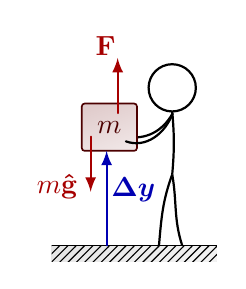
\begin{tikzpicture}
    \def\W{2.1}  % ground width
    \def\D{0.2}  % ground depth
    \def\h{0.6}  % mass height
    \def\w{0.7}  % mass width
    \def\H{2.0}  % human height
    \def\F{0.7}  % human height
    \def\mx{-0.15*\W} % mass x coordinate
    \def\my{ 0.60*\H} % mass y coordinate

    % PERSON
    \draw[thick] (0.23*\W,\H) circle (0.3) coordinate (H);
    \draw[thick] (H)++(-90:0.3) coordinate (N) to[out=-85,in=85]++ (0,-0.40*\H) coordinate (P);
    %\draw[thick,line cap=round] (N)++(-85:0.03) to[out=-115,in=3] (RH);
    \draw[thick,line cap=round] (N)++(-85:0.03) to[out=-120,in=-10] (\mx+0.3*\w,\my+0.3*\h); % right arm
    \draw[thick] (P) to[out=-110,in=85] (0.15*\W,0); % right leg (on the left)
    \draw[thick] (P) to[out=-80,in=108] (0.29*\W,0); % left leg (on the right)

    % SETUP
    \draw[ground] (-\W/2,0) rectangle++ (\W,-\D);
    \draw (-\W/2,0) --++ (\W,0);
    \draw[mass] (\mx-\w/2,\my) rectangle++ (\w,\h) node[midway] {$m$};
    \draw[thick,line cap=round] (N)++(-85:0.03) to[out=-110,in=-20] (\mx+0.3*\w,\my+0.2*\h); % right arm

    % FORCES
    %\draw[->] (0.42*\W,0.5*\h) --++ (0,0.9*\h) node[below=4,right=0] {$y$};
    \draw[force] (\mx+0.15*\w,\my+0.8*\h) --++ (0, \F) node[above left=-3] {$\vbF$};
    \draw[force] (\mx-0.34*\w,\my+0.3*\h) --++ (0,-\F) node[below=-2,left=1] {$m\vu{g}$};
    \draw[force,xcol] (\mx-0.05*\w,0) --++ (0,\my) node[midway,above=3,right=-2] {$\vb*{\Delta y}$};

\end{tikzpicture}


\end{document}